\documentclass[11pt]{article}

\usepackage[margin=1in]{geometry}
\usepackage{amsmath,amssymb}
\usepackage{booktabs}
\usepackage{graphicx}
\usepackage{hyperref}
\usepackage{array}
\newcolumntype{L}[1]{>{\raggedright\arraybackslash}p{#1}}

\emergencystretch=2em

\title{A Conservative Mimetic Polygon Interpolant on Nonmatching Voronoi Patches}
\author{Mimetic-SphPoly implementation notes}
\date{\today}

\newcommand{\uh}{\mathbf{u}_h}
\newcommand{\x}{\mathbf{x}}
\newcommand{\n}{\mathbf{n}}
\newcommand{\R}{\mathbb{R}}
\graphicspath{{docs/figures/}{figures/}}

\begin{document}
\maketitle

\begin{abstract}
This report documents the current C++14, MOAB, and Eigen3 prototype for conservative
mimetic interpolation on planar polygon patches.  The implementation follows
the level-2 truncated harmonic-polynomial reconstruction of Perot and Chartrand
\cite{PerotChartrand2021}.  Source data are signed edge-normal flux integrals.
For each source polygon, the code reconstructs a local vector field with
constant divergence and a curl-free cell interior.  The conservative transfer
property is verified by clipping nonmatching source and target polygon meshes
and checking the divergence theorem on every source-target intersection
polygon.  Current tests include a constant-field patch test, a nonmatching
rectangular mesh test, and a deterministic Voronoi n-gon patch test with source
and target cells having more than four sides.
\end{abstract}

\section{Scope and Current Status}

The implemented kernel is a planar prototype.  It is intended to be the
cell-local and overlap-local foundation for a later spherical implementation
using MOAB spherical mesh data and local tangent-plane or intrinsic spherical
geometry.  The current code does not yet implement spherical polygon
intersections, parallel ownership, or production spatial search.  Those are
separable extensions once the local mimetic reconstruction and overlap
conservation checks are stable.

The current repository contains:
\begin{itemize}
  \item \texttt{include/mimetic/mimetic.hpp}: public geometry, reconstruction,
        and reduction API.
  \item \texttt{src/mimetic.cpp}: implementation of the level-2 reconstruction,
        MOAB tag handling, line integrals, and polygon boundary fluxes.
  \item \texttt{tests/patch\_test.cpp}: constant-field patch test.
  \item \texttt{tests/conservative\_}\allowbreak\texttt{intersection\_test.cpp}:
        rectangular nonmatching source-target overlap test.
  \item \texttt{tests/voronoi\_}\allowbreak\texttt{intersection\_test.cpp}:
        deterministic Voronoi source-target n-gon overlap test.
  \item \texttt{docs/make\_report\_figures.py}: deterministic figure generator
        for the manuscript visualizations.
  \item \texttt{docs/figures/}: generated PDF figures included in the manuscript.
\end{itemize}

\section{Literature Survey}

Mimetic methods are built to preserve differential identities and physically
meaningful integral quantities at the discrete level.  The general philosophy is
reviewed by Bochev and Hyman \cite{BochevHyman2006}; a related finite element
viewpoint is finite element exterior calculus, where fields are associated with
geometric entities and de Rham complex structure is preserved
\cite{ArnoldFalkWinther2006}.  Mattiussi \cite{Mattiussi1997} provides an
algebraic-topological interpretation connecting finite volume, finite element,
and finite difference discretizations.

The local vector reconstruction used here is descended from low-order
H(div)-conforming mixed finite elements.  Raviart and Thomas introduced the
classical mixed element family for second-order elliptic problems
\cite{RaviartThomas1977}; Nedelec generalized compatible vector finite elements
for three-dimensional electromagnetic applications \cite{Nedelec1980}.  These
methods motivate storing normal flux degrees of freedom on faces or edges,
rather than storing Cartesian vector components at points.

Polygonal and polyhedral meshes require additional care because the number of
sides is not fixed.  Mimetic finite difference and support-operator methods
address this by designing discrete inner products directly
\cite{BrezziLipnikovSimoncini2005,LipnikovManziniShashkov2014}.  Virtual element
methods extend finite element ideas to polygonal cells by avoiding explicit
closed-form basis functions while preserving polynomial consistency and
stability \cite{BeiraoDaVeiga2013,BeiraoDaVeiga2016}.  The Perot-Chartrand
method can be interpreted in this family: it defines a computable local
reconstruction and a corresponding Hodge-like inner product from edge-normal
data \cite{PerotChartrand2021}.

The present tests use bounded Voronoi cells as realistic n-sided convex
polygons.  Voronoi diagrams are a standard way to create irregular polygonal
meshes \cite{Aurenhammer1991}.  The source-target intersection kernel in the
test uses repeated half-plane clipping, a direct specialization of the
Sutherland-Hodgman polygon clipping algorithm to convex polygons
\cite{SutherlandHodgman1974}.  MOAB supplies the mesh database abstraction and
tagged entity model used by the prototype \cite{Tautges2004}; Eigen3 supplies
the local dense linear algebra \cite{Eigen3}.

\section{Mathematical Method}

\subsection{Input and Output Data}

Let \(K\) be a source polygon with boundary edges \(f \subset \partial K\).
The discrete source field is the signed integrated normal flux
\begin{equation}
  U_f = \int_f \mathbf{u}\cdot\n_f\, ds,
  \label{eq:edge_flux}
\end{equation}
where \(\n_f\) is the outward unit normal of \(K\).  The output on a target edge
or an overlap boundary edge is another signed integral of the reconstructed
field.  Conservative interpolation is judged by exact agreement of integrated
fluxes on source-target intersections, not by pointwise vector agreement.

\subsection{Level-2 Harmonic Reconstruction}

In two dimensions the Perot-Chartrand reconstruction writes the cell field as
\begin{equation}
  \uh(\x) = \nabla\phi(\x) + \frac{d}{2}\x,
  \label{eq:pc_reconstruction}
\end{equation}
where \(d\) is constant in the cell and \(\phi\) is harmonic.  The implementation
uses a level-2 truncated harmonic polynomial basis,
\begin{align}
  P_1 &= x, & Q_1 &= y,\\
  P_2 &= x^2-y^2, & Q_2 &= 2xy,
  \label{eq:basis}
\end{align}
so that
\begin{equation}
  \uh(\x)
    = \frac{d}{2}\x
      + a_1\nabla P_1 + b_1\nabla Q_1
      + a_2\nabla P_2 + b_2\nabla Q_2.
  \label{eq:level2}
\end{equation}
All coordinates in the code are expressed in a centroid-relative local planar
frame.  This reduces low-order moment coupling and matches the assumptions used
in the paper's construction.

The constant divergence is fixed by the source fluxes:
\begin{equation}
  d = \frac{1}{|K|}\sum_{f\subset\partial K} U_f.
  \label{eq:divergence}
\end{equation}
For any scalar test function \(H\), Gauss' theorem gives
\begin{equation}
  \int_K \nabla H\cdot \mathbf{u}\,dA
  =
  \sum_{f\subset\partial K} U_f
  \left(\overline{H}_f-\overline{H}_K\right),
  \label{eq:moment}
\end{equation}
under the lowest-order assumption that the edge-normal data are constant per
edge.  In the code we subtract the known divergence contribution
\(\frac{d}{2}\x\) and solve the small harmonic system
\begin{equation}
  V\alpha = r,\qquad
  \alpha = (a_1,b_1,a_2,b_2)^T,
  \label{eq:local_system}
\end{equation}
where
\begin{equation}
  V_{ij} = \int_K \nabla H_i\cdot\nabla H_j\,dA
  \label{eq:gram}
\end{equation}
and
\begin{equation}
  r_i =
    \sum_{f\subset\partial K} U_f
      \left(\overline{H_i}_f-\overline{H_i}_K\right)
    - \frac{d}{2}\int_K \x\cdot\nabla H_i\,dA.
  \label{eq:rhs}
\end{equation}
Here \(H_i\in\{P_1,Q_1,P_2,Q_2\}\).  Equation
\eqref{eq:local_system} is solved with Eigen's dense LDLT solver.  Since the
current truncation has four harmonic unknowns, the solve cost is constant per
cell.

\subsection{Reduction and Conservative Overlap Integrals}

Because \(\uh\) is a gradient-form field plus \(\frac{d}{2}\x\), a line
integral from \(A\) to \(B\) can be evaluated exactly:
\begin{equation}
  \int_A^B \uh\cdot d\x
  =
  \frac{d}{4}\left(|B|^2-|A|^2\right)
  + \sum_i a_i\left(P_i(B)-P_i(A)\right)
  + \sum_i b_i\left(Q_i(B)-Q_i(A)\right).
  \label{eq:line_integral}
\end{equation}
For an overlap polygon \(O=K_s\cap K_t\), the conservative property is tested by
integrating the outward-normal flux around the overlap boundary:
\begin{equation}
  \int_{\partial O} {\uh}_s\cdot\n\,ds = d_s |O|.
  \label{eq:overlap_conservation}
\end{equation}
This is the local divergence theorem.  It is the key invariant that a
conservative source-to-target interpolation must satisfy on every intersection
region.

\subsection{Edge-wise Source-to-Target Transfer}

The overlap diagnostic above is necessary but not sufficient for a usable edge
remap.  A target edge degree of freedom must be computed on the target edge
itself.  For a directed target edge \(e_t=[A,B]\) with target outward normal
\(\n_t\), the implemented transfer clips the edge against every source cell and
sums the source-cell contributions:
\begin{equation}
  U^t_{e_t}
  =
  \sum_{K_s:\, e_t\cap K_s\neq\emptyset}
  \int_{e_t\cap K_s} {\uh}_{K_s}\cdot\n_t\,ds .
  \label{eq:edge_transfer}
\end{equation}
The segment orientation is inherited from the target cell boundary, so the
normal in Eq.~\eqref{eq:edge_transfer} is the target-cell normal rather than the
source-cell normal.  This is the edge-wise source-to-target transfer that the
current nonmatching tests now validate.

The map is linear in the source edge fluxes.  For each source cell \(K_s\), the
local reconstruction can be written
\begin{equation}
  \beta_{K_s}=B_{K_s}U_{K_s},
  \qquad
  \beta_{K_s}=(d,a_1,b_1,a_2,b_2)^T,
  \label{eq:local_reconstruction_matrix}
\end{equation}
and each clipped target-edge segment defines a row functional
\(L_{\gamma,K_s}\).  The assembled sparse projection is therefore
\begin{equation}
  U_t = P U_s,\qquad
  P_{e_t,f_s} \mathrel{+}=
  L_{\gamma,K_s} B_{K_s}(:,f_s).
  \label{eq:sparse_projection}
\end{equation}
Rows of \(P\) are directed target-cell edges, and columns are directed
source-cell edges.  This directed convention is important because normal flux
orientation is cell-local; a shared undirected mesh edge needs a separate
orientation map before edge DOFs are collapsed.

\section{Algorithms and Code Traceability}

\subsection*{Algorithm 1: Source-Cell Reconstruction}
\begin{enumerate}
  \item Extract ordered MOAB polygon connectivity.
  \item Enforce counter-clockwise orientation and shift coordinates by the cell
        centroid.
  \item Create ordered local edges and outward normals.
  \item Read \(U_f\) from the \texttt{SOURCE\_FLUX} edge tag.
  \item Compute \(d\) from Eq.~\eqref{eq:divergence}.
  \item Assemble \(V\) using Eq.~\eqref{eq:gram}.
  \item Assemble \(r\) using Eq.~\eqref{eq:rhs}.
  \item Solve \(V\alpha=r\) and store \((c,d,a_1,b_1,a_2,b_2)\) in
        \texttt{COEFFS}.
\end{enumerate}

\subsection*{Algorithm 2: Conservative Evaluation on a Target or Overlap Edge}
\begin{enumerate}
  \item Convert target or overlap vertices into the source-cell local frame.
  \item For line integrals use Eq.~\eqref{eq:line_integral}.
  \item For overlap conservation, integrate each directed overlap boundary edge
        with the outward normal implied by counter-clockwise order.
  \item Sum edge contributions and compare to \(d_s |O|\).
\end{enumerate}

\subsection*{Algorithm 3: Voronoi Patch Verification}
\begin{enumerate}
  \item Generate source and target bounded Voronoi cells by clipping the unit
        square with perpendicular bisectors.
  \item Create MOAB polygons for all nondegenerate cells.
  \item Set analytic source edge fluxes from \(\mathbf{u}(x,y)=(x,y)\).
  \item Reconstruct every source cell using Algorithm 1.
  \item Clip each source-target pair using convex polygon clipping.
  \item For every nonempty overlap, check Eq.~\eqref{eq:overlap_conservation}.
  \item For every target cell, check that source overlaps cover the target area
        and that the overlap-summed conservative integral equals \(2|K_t|\).
\end{enumerate}

\subsection*{Algorithm 4: Directed Edge Transfer and Sparse Projection}
\begin{enumerate}
  \item Enumerate directed source-cell edge DOFs and directed target-cell edge
        DOFs.
  \item For each source cell, build \(B_{K_s}\) from
        Eq.~\eqref{eq:local_reconstruction_matrix}.
  \item For each directed target edge, clip the target segment against every
        source polygon.
  \item For direct transfer, evaluate Eq.~\eqref{eq:edge_transfer} on each
        clipped segment and sum into the target edge flux tag.
  \item For matrix assembly, apply the segment functional to \(B_{K_s}\) and add
        triplets to the global sparse matrix \(P\) in Eq.~\eqref{eq:sparse_projection}.
  \item Store \(P\) in MatrixMarket coordinate format and write CSV maps for row
        and column DOFs.
\end{enumerate}

\begin{center}
\small
\begin{tabular}{@{}L{0.24\linewidth}L{0.31\linewidth}L{0.35\linewidth}@{}}
\toprule
Manuscript object & Code location & Purpose \\
\midrule
\(P_1,Q_1,P_2,Q_2\) and gradients &
\texttt{p1}, \texttt{q1}, \texttt{p2}, \texttt{q2}, \texttt{grad\_*} in
\texttt{mimetic.hpp/cpp} &
Implements Eq.~\eqref{eq:basis}. \\
\(U_f\) &
\texttt{SOURCE\_FLUX} tag exposed by
\texttt{MimeticInterpolator::}\newline\texttt{source\_flux\_tag()} &
Signed source-edge integrated normal flux. \\
\(d\) &
\texttt{ReconstructionCoeffs::d} &
Constant divergence from Eq.~\eqref{eq:divergence}. \\
\(V\alpha=r\) &
\texttt{MimeticInterpolator::}\newline\texttt{reconstruct\_source\_polygon()} &
Builds Eqs.~\eqref{eq:gram}--\eqref{eq:rhs} and solves Eq.~\eqref{eq:local_system}. \\
\(\int_A^B\uh\cdot d\x\) &
\texttt{MimeticInterpolator::}\newline\texttt{line\_integral()} &
Implements Eq.~\eqref{eq:line_integral}. \\
\(\int_{\partial O}\uh\cdot\n ds\) &
\texttt{MimeticInterpolator::}\newline\texttt{polygon\_boundary\_flux()} &
Overlap conservation diagnostic in Eq.~\eqref{eq:overlap_conservation}. \\
Voronoi cells &
\texttt{voronoi\_cell\_polygon()} in
\texttt{voronoi\_intersection\_}\newline\texttt{test.cpp} &
Creates n-sided bounded Voronoi cells by half-plane clipping. \\
Source-target overlap &
\texttt{convex\_intersection()} in
\texttt{voronoi\_intersection\_}\newline\texttt{test.cpp} &
Computes \(K_s\cap K_t\) for convex polygon pairs. \\
Target edge transfer &
\texttt{transfer\_source\_to\_}\newline\texttt{target\_edges()} &
Implements Eq.~\eqref{eq:edge_transfer} by clipping each target edge by source
cells. \\
Sparse projection &
\texttt{assemble\_edge\_projection\_}\newline\texttt{operator()} and
\texttt{write\_matrix\_market()} &
Builds and writes the directed edge map in Eq.~\eqref{eq:sparse_projection}. \\
\bottomrule
\end{tabular}
\end{center}

\section{Algorithmic Analysis}

Let \(n_K\) be the number of sides of one polygon and let \(q=4\) be the number
of harmonic coefficients in the current level-2 truncation.

\paragraph{Local reconstruction.}
Geometry extraction and edge moment evaluation are \(O(n_K)\).  Assembly of
the Gram matrix is \(O(q^2 n_K)\), and assembly of the right-hand side is
\(O(q n_K)\).  The dense solve is \(O(q^3)\).  Since \(q=4\) is fixed, the
reconstruction cost is effectively linear in the number of polygon sides:
\[
  T_{\mathrm{recon}}(K)=O(n_K).
\]

\paragraph{Overlap evaluation.}
For convex source and target polygons with \(n_s\) and \(n_t\) sides, repeated
half-plane clipping costs \(O(n_s n_t)\) in the simple implementation used by
the test.  Once an overlap polygon \(O\) with \(n_O\) sides is known, the
boundary-flux check is \(O(n_O)\).  In production, the all-pairs source-target
loop should be replaced by a spatial index or advancing-front intersection
algorithm; the current test intentionally uses direct all-pairs clipping for
clarity and reproducibility.

\paragraph{Edge transfer and projection assembly.}
Let \(E_t\) be the number of directed target edges and \(N_s\) the number of
source cells.  The current all-pairs implementation clips each target edge
against each source polygon, so its cost is \(O(E_t N_s \bar n_s)\) for average
source side count \(\bar n_s\).  Sparse matrix assembly has the same geometric
cost plus local coefficient-row multiplication.  The number of nonzeros is
proportional to the number of source-edge basis functions that influence each
clipped target-edge segment.

\paragraph{Memory.}
Each source cell stores six doubles in \texttt{COEFFS}.  Each source or target
edge stores one double flux tag.  Temporary dense matrices are \(4\times4\) and
are allocated per reconstructed source cell.  The sparse projection stores
directed source and target edge maps plus compressed sparse matrix arrays.

\section{Results and Discussion}

All results below were produced by:
\begin{verbatim}
cmake -S . -B /tmp/mimetic-sphpoly-build
cmake --build /tmp/mimetic-sphpoly-build --parallel
ctest --test-dir /tmp/mimetic-sphpoly-build --output-on-failure
env MPLCONFIGDIR=/tmp/mimetic-sphpoly-mpl python3 docs/make_report_figures.py
\end{verbatim}

\subsection{Visualization of the Overlap Geometry}

Figure~\ref{fig:rectangular-overlap} shows the simplest nonmatching transfer
geometry.  The source mesh has four cells, the target mesh has nine cells, and
their overlay creates 16 nonempty source-target intersections.  This case is
useful because every clipped region is a rectangle, so area and boundary flux
can be checked independently of any complicated polygon clipping.

\begin{figure}[t]
  \centering
  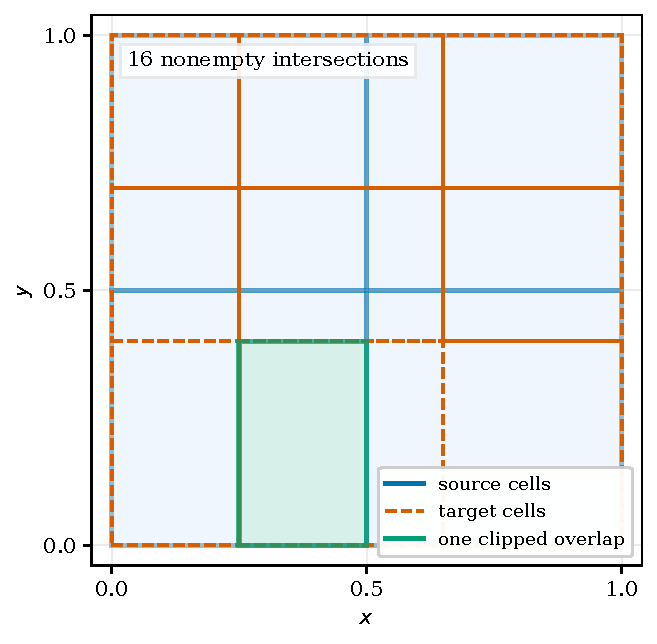
\includegraphics[width=0.68\linewidth]{rectangular_overlap.pdf}
  \caption{Rectangular source-target overlay.  Blue cells are the \(2\times2\)
  source mesh, dashed orange cells are the nonmatching \(3\times3\) target mesh,
  and the green rectangle is one clipped source-target intersection.}
  \label{fig:rectangular-overlap}
\end{figure}

Figure~\ref{fig:voronoi-patch} shows the more relevant polygonal case: two
bounded Voronoi meshes with different seeds and different side counts.  The
source mesh contains seven cells with more than four sides; those cells are
marked by their side count.  The target mesh contains ten cells with more than
four sides.  The visual point of this test is that the reconstruction and
conservative reduction are exercised on genuine n-sided polygons rather than on
quadrilateral cells.

\begin{figure}[t]
  \centering
  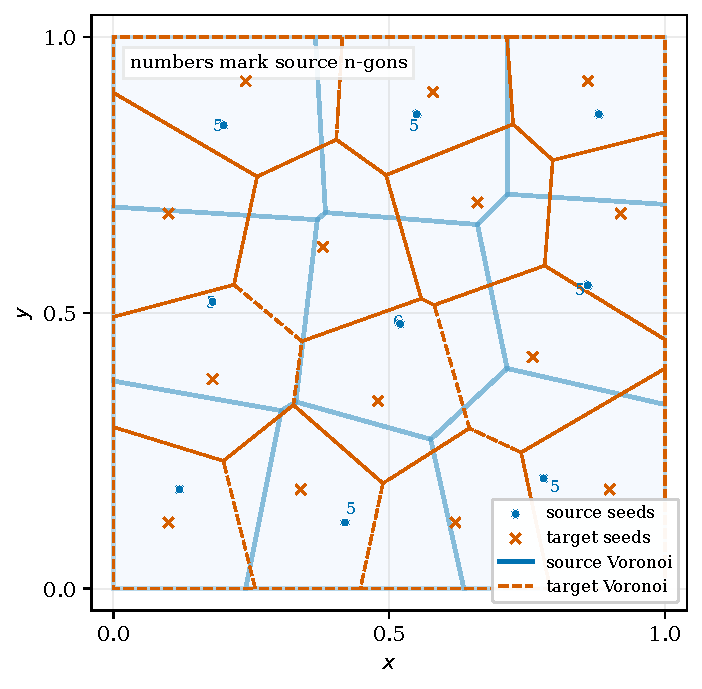
\includegraphics[width=0.70\linewidth]{voronoi_patch.pdf}
  \caption{Nonmatching bounded Voronoi patch.  Blue polygons are source cells
  and dashed orange polygons are target cells.  The numbers mark source cells
  with \(n>4\) sides.}
  \label{fig:voronoi-patch}
\end{figure}

Figure~\ref{fig:voronoi-overlap-detail} isolates one source-target pair in
which both cells have more than four sides.  The green polygon is the clipped
intersection \(O=K_s\cap K_t\).  In the test, the conservative flux check is
performed on this clipped polygon and on every other nonempty overlap.

\begin{figure}[t]
  \centering
  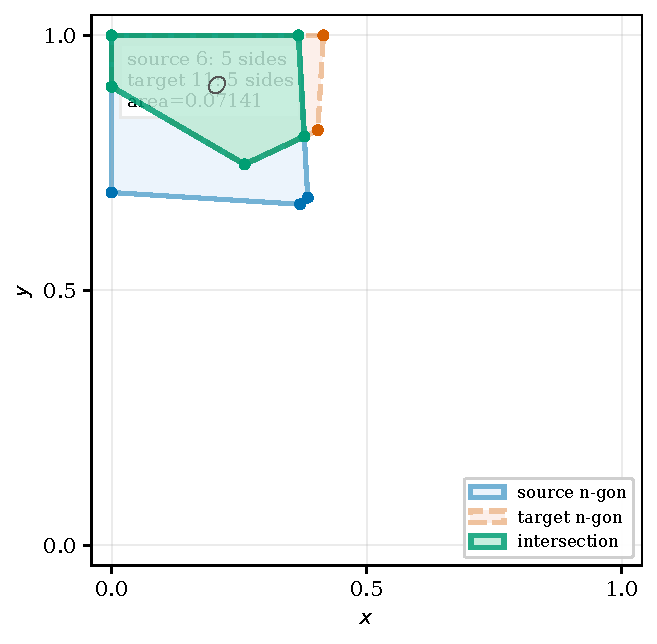
\includegraphics[width=0.68\linewidth]{voronoi_overlap_detail.pdf}
  \caption{Example n-gon to n-gon overlap.  The conservative diagnostic
  integrates the reconstructed source field around the green intersection
  boundary and compares it with \(d_s|O|\).}
  \label{fig:voronoi-overlap-detail}
\end{figure}

\subsection{Constant-Field Patch Test}

The patch test uses a unit-square source cell and an interior nonmatching target
quadrilateral.  With analytic field \(\mathbf{u}=(1,1)\), the reconstruction
recovers
\[
  d=0,\qquad a_1=1,\qquad b_1=1,\qquad a_2=b_2=0
\]
to roundoff.  The interior line integral from
\((-0.2,-0.3)\) to \((0.4,0.2)\) in source-local coordinates is exactly \(1.1\).
The target edge fluxes are \((-0.55,0.55,0.55,-0.55)\), and their sum is zero.
The maximum printed absolute error in the coefficient, line-integral, and target
edge checks is zero at the displayed precision.

\subsection{Rectangular Nonmatching Mesh Test}

The rectangular test uses a \(2\times2\) source grid and a nonmatching \(3\times3\)
target grid over the same unit square.  The analytic source field is
\(\mathbf{u}=(x,y)\), so \(\nabla\cdot\mathbf{u}=2\).  The test checks every one
of the 16 source-target rectangular intersections.  Each overlap satisfies
Eq.~\eqref{eq:overlap_conservation} to roundoff.  The aggregate overlap area is
1 and the aggregate divergence integral is 2.
The largest printed per-overlap boundary-flux error is
\(2.78\times10^{-17}\).  The aggregate source-target area error is
\(2.22\times10^{-16}\), and the aggregate integral error relative to
\(\int_\Omega\nabla\cdot(x,y)\,dA=2\) is \(4.44\times10^{-16}\).
The edge-wise transfer then computes 36 directed target edge fluxes.  Each
target edge agrees with the analytic integral of \(\mathbf{u}(x,y)=(x,y)\) to
roundoff, and each target cell satisfies
\[
  \sum_{e_t\subset\partial K_t} U^t_{e_t}=2|K_t|.
\]
The assembled sparse projection for this case has 36 rows, 16 columns, and 80
nonzeros.  Applying this matrix to the directed source edge flux vector
reproduces the direct edge-transfer result to roundoff, and the matrix is
written to MatrixMarket format with source and target edge-map CSV files.

\subsection{Voronoi n-gon Patch Test}

The Voronoi test uses two different bounded Voronoi meshes over the unit square.
The source mesh side-count histogram is
\[
  n=4:2,\qquad n=5:6,\qquad n=6:1,
\]
so seven source cells have more than four sides.  The target mesh side-count
histogram is
\[
  n=4:4,\qquad n=5:5,\qquad n=6:5,
\]
so ten target cells have more than four sides.  The source-target clipping
produces 36 nonempty overlaps, including 23 n-gon to n-gon overlaps where both
the source and target cells have more than four sides.

Every overlap satisfies Eq.~\eqref{eq:overlap_conservation}.  Each target cell
is covered by source overlaps to roundoff.  The aggregate checks are:
\[
  \sum |K_s\cap K_t| = 1,\qquad
  \sum \int_{\partial(K_s\cap K_t)}{\uh}_s\cdot\n\,ds = 2,\qquad
  \int_\Omega \nabla\cdot(x,y)\,dA = 2.
\]
The largest printed overlap or aggregate residual is \(4.44\times10^{-16}\),
well below the \(5\times10^{-10}\) tolerance used for the summed Voronoi flux
check.  Figure~\ref{fig:results-summary} summarizes the Voronoi coverage counts
and the conservation residual scale across the three tests.
The edge-wise Voronoi transfer computes 71 directed target edge fluxes.  Every
target edge agrees with the analytic global linear field integral to roundoff,
and every target cell satisfies the same edge-flux divergence check
\(\sum U^t_{e_t}=2|K_t|\).

\begin{figure}[t]
  \centering
  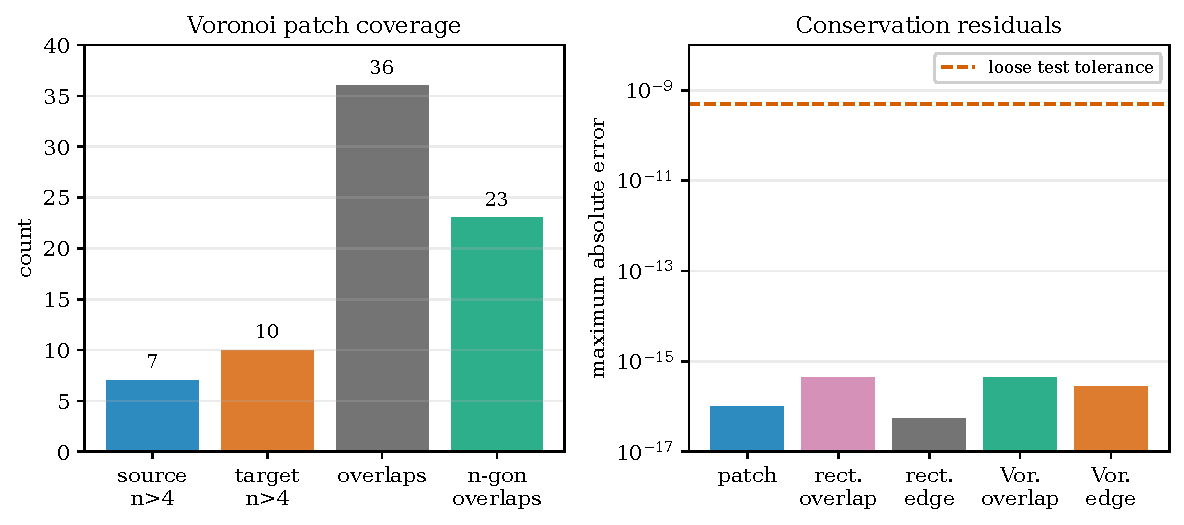
\includegraphics[width=0.92\linewidth]{results_summary.pdf}
  \caption{Summary of verification coverage and conservation residuals.  The
  patch-test residual is plotted at \(10^{-16}\) to show it on the logarithmic
  scale; the printed test output reports zero at displayed precision.}
  \label{fig:results-summary}
\end{figure}

\begin{table}[t]
  \centering
  \small
  \begin{tabular}{@{}L{0.24\linewidth}L{0.34\linewidth}L{0.22\linewidth}L{0.12\linewidth}@{}}
  \toprule
  Test & Geometry exercised & Strongest checked invariant & Observed residual \\
  \midrule
  Constant patch &
  One source quadrilateral and one contained target quadrilateral &
  Constant field coefficients and closed target-edge flux sum &
  \(0\) printed \\
  Rectangular overlay &
  Four source cells, nine target cells, 16 clipped intersections &
  Overlap conservation, 36 directed target edge fluxes, and 36-by-16 sparse
  projection application &
  \(4.44\times10^{-16}\) \\
  Voronoi n-gon overlay &
  Nine source cells, 14 target cells, 36 overlaps, 23 n-gon to n-gon overlaps &
  Same overlap invariant plus 71 directed target edge fluxes &
  \(4.44\times10^{-16}\) \\
  \bottomrule
  \end{tabular}
  \caption{Verification summary from the current CTest runs.  Residuals are
  absolute errors reported by the deterministic regression tests.}
  \label{tab:verification-summary}
\end{table}

\subsection{Discussion}

The results show that the conservative property is controlled by three local
ingredients: exact reconstruction of the polynomial moments used by the
level-2 basis, exact reduction over each clipped overlap boundary, and
edge-wise target-segment clipping with the target edge normal.  For the
manufactured field \(\mathbf{u}=(x,y)\), the reconstructed divergence is
constant and equal to 2 on every source cell.  Therefore the expected overlap
flux is \(2|O|\), and the target-cell edge flux sum is \(2|K_t|\).  The
residuals in Table~\ref{tab:verification-summary} measure only floating-point
and clipping-roundoff effects.

The Voronoi test is the most informative current result.  It rules out a common
false positive in polygon remapping prototypes: passing only quadrilateral or
axis-aligned cases.  Here both source and target meshes contain five- and
six-sided cells, and 23 nonempty intersections involve n-gons on both sides.
The exact overlap identity holds on each of those intersections, which is the
local condition needed before adding spatial acceleration, parallel ownership,
or spherical geometry.  The new directed-edge checks additionally verify that
the remapped edge data themselves, not only overlap-cell diagnostics, reproduce
the analytic target edge integrals.

The visualizations also clarify what is not yet tested.  The clipping kernel is
currently convex and planar; it does not cover nonconvex polygons, spherical
great-circle arcs, or overlaps crossing a projection singularity.  Those
extensions should preserve the same acceptance criterion,
Eq.~\eqref{eq:overlap_conservation}, but they will need geometry-specific
intersection and quadrature tests.

\section{Assumptions and Limitations}

\begin{itemize}
  \item The implementation is currently planar.  Spherical meshes require a
        documented choice of geometry: local tangent-plane approximation,
        gnomonic projection, or intrinsic spherical polygon integration.
  \item The reconstruction is level-2 only.  This is the practical stable choice
        emphasized by Perot and Chartrand for polygon meshes
        \cite{PerotChartrand2021}, but level-3 diagnostics may be useful for
        severe distortion or high valence.
  \item Convex clipping is implemented in the Voronoi test only.  A production
        source-target transfer should move this to the library and pair it with
        MOAB spatial search.
  \item Tests use manufactured analytic fields and exact planar overlap
        geometry.  They verify local conservation and reconstruction
        consistency, not global PDE accuracy.
  \item The current source-target transfer routine for target edges assumes a
        target polygon contained in one source cell.  General nonmatching meshes
        should use \texttt{transfer\_source\_to\_}\allowbreak\texttt{target\_edges()}
        or the sparse projection assembly path.
  \item The sparse projection currently uses directed cell-edge DOFs.  Shared
        mesh-edge collapse requires explicit orientation metadata.
\end{itemize}

\section{Conclusions}

The present implementation demonstrates that the level-2 harmonic-polynomial
mimetic reconstruction can be expressed cleanly in MOAB/Eigen3 and verified on
nonmatching polygon patches.  The strongest current result is the Voronoi n-gon
test: it exercises genuine five- and six-sided source and target cells, clips
all nonempty source-target intersections, verifies the conservative overlap
identity on every region, and computes 71 directed target edge fluxes.  The
rectangular test also assembles and writes an explicit sparse directed
source-edge to target-edge projection matrix.  This validates the core local
reconstruction, edge-wise remap, and local conservative integration kernels
needed for a future spherical polygon mesh transfer tool.

The next implementation phase should move convex polygon intersection into the
library, add MOAB spatial acceleration, and then introduce spherical geometry.
At that point the same overlap invariant, Eq.~\eqref{eq:overlap_conservation},
should remain the primary acceptance test.

\bibliographystyle{plain}
\bibliography{references}

\end{document}
